\documentclass[xcolor=svgnames]{beamer}
\usetheme{Torino}

\usepackage{epsfig} %for figures
\usepackage{xcolor} %for color
\usepackage[utf8]{inputenc}
\usepackage{multicol}
\usepackage{hyperref}
\setbeamertemplate{footline}[frame number]

% latex definitions:
\def\d{{\rm d}}
\def\half{{\textstyle{1\over2}}}



\title[SymPy\hspace{4em}\insertframenumber/
\inserttotalframenumber]{~\\ SymPy Tutorial \\~}


\author[A. Meurer, S.Y. Lee]
{Aaron Meurer, S.Y. Lee}

\pgfdeclareimage[height=1.5cm]{mylogo}{sympy-logo}
\institute{\pgfuseimage{mylogo}}

\date{July 11, 2023}

\begin{document}

\begin{frame}
  \maketitle
\begin{center}
\normalsize All materials for today's tutorial are at \url{https://www.sympy.org/scipy-2023-tutorial/}
\end{center}
\end{frame}

\begin{frame}{Who are we?}
  \begin{block}{Aaron Meurer}
    \begin{center}
      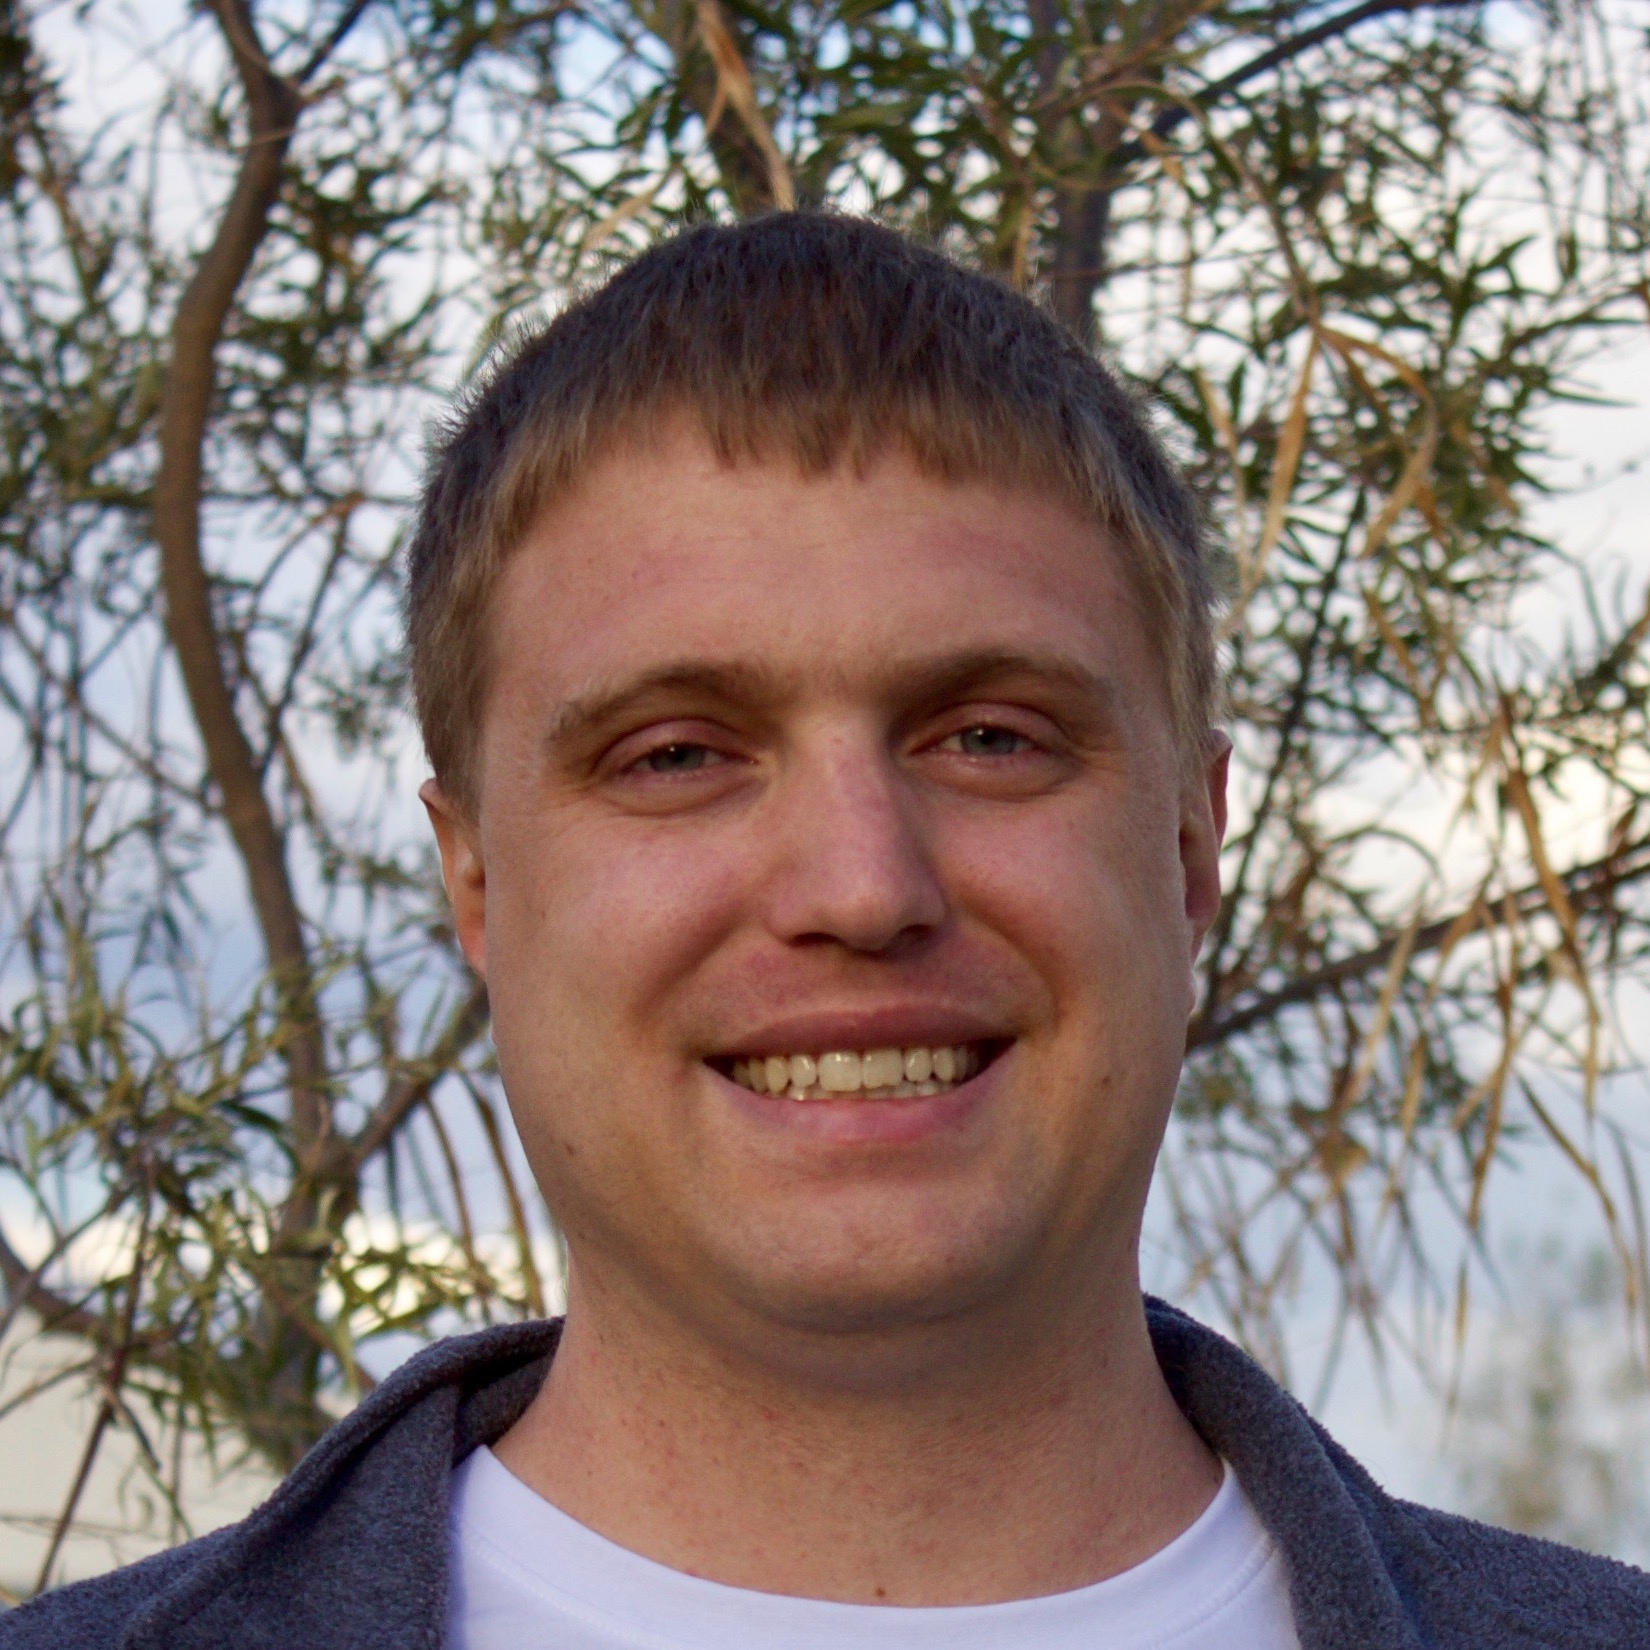
\includegraphics[height=3.5cm]{aaron.png}
    \end{center}
    I am a software engineer at Quansight. I have contributed to SymPy since
    2009. I have also contributed to various projects in the array API
    ecosystem.
    \\
    I will be giving a talk at the conference ``Python Array API Standard'' on
    Friday at 11:25–11:55 in Amphitheater 204. Please come if you are
    interested.
  \end{block}
\end{frame}

\begin{frame}{Who are we?}
  \begin{block}{S.Y Lee}
    \begin{center}
      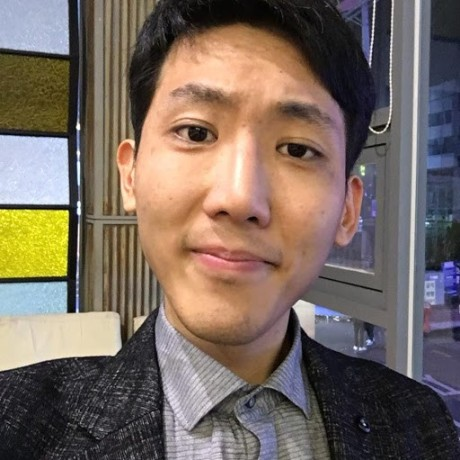
\includegraphics[height=3.5cm]{sylee.jpeg}
    \end{center}
    I am a freelance software engineer at \href{https://mathpix.com/}{Mathpix}.
    I have worked on frontend mathematical systems in Python and Typescript,
    with \href{https://www.tigermilk.education/}{TigerMilk.Education} and \href{https://mathpresso.com/}{QANDA Team}
  \end{block}
\end{frame}

\begin{frame}
  \begin{block}{What is SymPy?}
\begin{itemize}
    \item SymPy is a pure Python library for \textbf{symbolic mathematics} (as
      opposed to \textit{numerical mathematics}).
\item Symbolic mathematics is exact mathematics, like you would do on a chalkboard.
      \item For example, the difference between computing $\sqrt{8}\approx
        2.82842712474619$ and $\sqrt{8}=2\sqrt{2}$.
\item SymPy supports a large number of areas of mathematics. We will only
  cover the basics in this tutorial. See the documentation (\href{https://docs.sympy.org/latest/index.html}{docs.sympy.org})
  for more.
\end{itemize}
    \end{block}
\end{frame}

\begin{frame}{SymPy Example}
  \begin{block}{}
    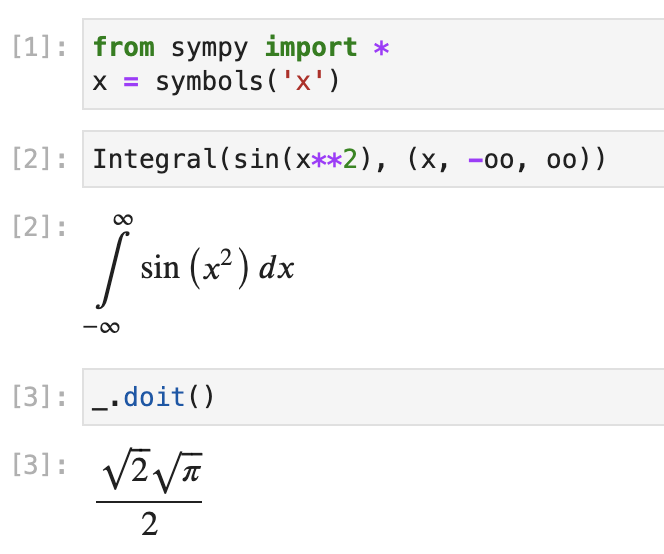
\includegraphics[height=6cm]{example.png}
  \end{block}
\end{frame}

\begin{frame}{SymPy Goal}
  \begin{block}{Goal}
    Provide a symbolic manipulation library in Python.
  \end{block}
  \begin{block}

    ``SymPy is an open source Python library for symbolic mathematics. It aims to
    become a full-featured computer algebra system (CAS) while keeping the code as
    simple as possible in order to be comprehensible and easily extensible. SymPy
    is written entirely in Python and does not require any external libraries.''

  \end{block}
\end{frame}

\begin{frame}{Why SymPy?}
  \begin{block}{}
    \begin{itemize}
      \item Standalone
      \item Full featured
      \item BSD licensed
      \item Embraces Python
      \item Usable as a library
    \end{itemize}
  \end{block}
\end{frame}

\begin{frame}{Features}
  \begin{multicols}{2}
    \tiny
    \begin{itemize}
    \item \textbf{Core Capabilities}
      \begin{itemize}
        \tiny
      \item Basic arithmetic: Support for operators such as +, -, *, /, ** (power)
      \item Simplification
      \item Expansion
      \item Functions: trigonometric, hyperbolic, exponential, roots, logarithms,
        absolute value, spherical harmonics, factorials and gamma functions, zeta
        functions, polynomials, special functions, \ldots
      \item Substitution
      \item Numbers: arbitrary precision integers, rationals, and floats
      \item Noncommutative symbols
      \item Pattern matching
      \end{itemize}
    \item \textbf{Polynomials}
      \begin{itemize}
        \tiny
      \item Basic arithmetic: division, gcd, \ldots
      \item Factorization
      \item Square-free decomposition
      \item Gröbner bases
      \item Partial fraction decomposition
      \item Resultants
      \end{itemize}
    \item \textbf{Calculus}
      \begin{itemize}
        \tiny
      \item Limits: $\lim_{x\to 0}{x\log(x)} = 0$
      \item Differentiation
      \item Integration
      \item Taylor (Laurent) series
      \end{itemize}
    \item \textbf{Solving equations}
      \begin{itemize}
        \tiny
      \item Polynomial equations
      \item Algebraic equations
      \item Differential equations
      \item Difference equations
      \item Systems of equations
      \end{itemize}
    \item \textbf{Combinatorics}
      \begin{itemize}
        \tiny
      \item Permutations
      \item Combinations
      \item Partitions
      \item Subsets
      \item Permutation Groups: Polyhedral, Rubik, Symmetric, \ldots
      \item Prufer and Gray Codes
      \end{itemize}

    \end{itemize}
  \end{multicols}
\end{frame}

\begin{frame}{Features}
  \begin{multicols}{2}
    \begin{itemize}
      \tiny
    \item \textbf{Discrete math}
      \begin{itemize}
        \tiny
      \item Binomial coefficients
      \item Summations
      \item Products
      \item Number theory: generating prime numbers, primality testing, integer
        factorization, \ldots
      \item Logic expressions
      \end{itemize}

    \item \textbf{Matrices}
      \begin{itemize}
        \tiny
      \item Basic arithmetic
      \item Eigenvalues/eigenvectors
      \item Determinants
      \item Inversion
      \item Solving
      \item Abstract expressions
      \end{itemize}


    \item \textbf{Geometry}
      \begin{itemize}
        \tiny
      \item points, lines, rays, segments, ellipses, circles, polygons, \ldots
      \item Intersection
      \item Tangency
      \item Similarity
      \end{itemize}

    \item \textbf{Plotting}
      \begin{itemize}
        \tiny
      \item Coordinate modes
      \item Plotting Geometric Entities
      \item 2D and 3D
      \item Interactive interface
      \item Colors
      \end{itemize}

    \item \textbf{Physics}
      \begin{itemize}
        \tiny
      \item Units
      \item Mechanics
      \item Quantum
      \item Gaussian Optics
      \item Pauli Algebra
      \end{itemize}

    \item \textbf{Statistics}
      \begin{itemize}
        \tiny
      \item Normal distributions
      \item Uniform distributions
      \item Probability
      \end{itemize}

    \item \textbf{Printing}
      \begin{itemize}
        \tiny
      \item Pretty printing: ASCII/Unicode pretty printing, LaTeX
      \item Code generation: C, Fortran, Python
      \end{itemize}
    \end{itemize}
  \end{multicols}
\end{frame}

\begin{frame}{Use Cases}
  \begin{block}{}
    \begin{itemize}
      \item Education (useful for both teachers and students)
      \item Calculator
      \item Scientific Modeling
      \item Code Generation
      \item SymPy is used in virtually every scientific field
    \end{itemize}
  \end{block}
\end{frame}

\begin{frame}{Present}
  \begin{block}{Current Status}
    \begin{itemize}
    \item Over 1200 contributors.
    \item $\sim$A dozen active core developers.
    \item Current code base has over 690,000 lines of code and documentation.
    \item Over 500 pull requests merged in the last year.
    \end{itemize}
  \end{block}
\end{frame}

\begin{frame}{Present}
  \begin{block}{Chan Zuckerberg Initiative Funding}
    CZI grant is funding core developers to improve
    \begin{itemize}
    \item Performance
    \item Documentation
    \item Code Generation
    \end{itemize}
  \end{block}
\end{frame}

\begin{frame}{Google Summer of Code}
  These are our current GSoC projects. Expect to see these features by the end
  of the summer.
  \begin{itemize}
  \item Ishan Pandhare: Extending Continuum mechanics module: Introducing classes for Cables and Improving the Truss class
  \item Tilo Reneau-Cardoso: Improving Relational Assumptions in SymPy’s New Assumptions
  \item Abhishek Patidar: Improving Polynomial GCD
  \item Tirthankar Mazumder: Rewrite LaTeX Parser
  \item Anurag Surendra Bhat: Improving And Expanding Functionalities Of SymPy's Control Module
  \end{itemize}
\end{frame}


\begin{frame}{Projects Using SymPy}
\begin{itemize}
\item
  \href{http://www.sagemath.org/}{\textbf{Sage}}: A CAS, visioned to be
  a viable free open source alternative to Magma, Maple, Mathematica and
  MATLAB\@. Sage includes many open source mathematical libraries, including
  SymPy.
\item
  \href{https://cloud.sagemath.com}{\textbf{SageMathCloud}}:
  SageMathCloud is a web-based cloud computing and course management
  platform for computational mathematics.
\item
  \href{http://www.pydy.org/}{\textbf{PyDy}}: Multibody Dynamics with
  Python.
\item
  \href{https://pytorch.org/docs/stable/dynamo/index.html}{\textbf{TorchDynamo}}:
  TorchDynamo is a Python-level JIT compiler designed to make unmodified
  PyTorch programs faster. It uses SymPy for its internal representation of
  array indexing expressions.
\end{itemize}
  \end{frame}

\begin{frame}{Projects Using SymPy}
\begin{itemize}
\item
  \href{http://octave.sourceforge.net/symbolic/}{\textbf{Octave Symbolic}}:
  The Octave-Forge Symbolic package adds symbolic calculation features
  to GNU Octave. These include common CAS tools such
  as algebraic operations, calculus, equation solving, Fourier and
  Laplace transforms, variable precision arithmetic, and other features.
\item
  \href{https://github.com/pygae/galgebra}{\textbf{galgebra}}:
  Geometric algebra (previously \texttt{sympy.galgebra}).
\item
  \href{https://github.com/jverzani/SymPy.jl}{\textbf{SymPy.jl}}:
  Provides a Julia interface to SymPy using PyCall.
\item
  \href{https://mathics.github.io/}{\textbf{Mathics}}: Mathics is a
  free, general-purpose online CAS featuring Mathematica compatible
  syntax and functions. It is backed by highly extensible Python code,
  relying on SymPy for most mathematical tasks.
\item
  \href{http://sfepy.org/}{\textbf{SfePy}}: Simple finite elements in
  Python.
\item
  \href{https://yt-project.org/}{\textbf{yt}}: Python package for
  analyzing and visualizing volumetric data
  (\href{https://unyt.readthedocs.io/en/stable/}{\textbf{unyt}}, the yt unit
  system, uses SymPy).
\end{itemize}
\end{frame}

\begin{frame}{Tutorial Outline}
  \begin{block}{}
    \begin{itemize}
\item Introduction to SymPy (presentation) (10 min.)

\item Introduction to Symbolic Computation (20 min.)

\item Basic operations (20 min.)

\item Break (10 min.)

\item Simplification (25 min.)

\item Calculus (25 min.)

\item Break (10 min.)

\item Matrices (25 min.)

\item Advanced expression manipulation (25 min.)

\item Break (10 min.)

\item Code Generation (30 min.)

\item Advanced Topics (30 min.)
    \end{itemize}
  \end{block}
\end{frame}

\begin{frame}
\Huge Let's begin!
\end{frame}
\end{document}
